%===============================================================================
% LaTeX sjabloon voor de bachelorproef toegepaste informatica aan HOGENT
% Meer info op https://github.com/HoGentTIN/bachproef-latex-sjabloon
%===============================================================================

\documentclass{bachproef-tin}

\usepackage{hogent-thesis-titlepage} % Titelpagina conform aan HOGENT huisstijl
\usepackage{svg}
\usepackage{tcolorbox}
\usepackage{tikz}
\usetikzlibrary{positioning}
\usetikzlibrary{decorations.pathreplacing,calligraphy}
\usepackage{float}

%%---------- Documenteigenschappen ---------------------------------------------

% De titel van het rapport/bachelorproef
\title{Integratie van blockchain binnen een zelfontwikkeld ERP-systeem}

% Je eigen naam
\author{Arno Temmerman}

% De naam van je promotor (lector van de opleiding)
\promotor{Jan Willem}

% De naam van je co-promotor. Als je promotor ook je opdrachtgever is en je
% dus ook inhoudelijk begeleidt (en enkel dan!), mag je dit leeg laten.
\copromotor{Geert Borloo}

% Indien je bachelorproef in opdracht van/in samenwerking met een bedrijf of
% externe organisatie geschreven is, geef je hier de naam. Zoniet laat je dit
% zoals het is.
\instelling{14IT}

% Academiejaar
\academiejaar{2021-2022}

% Examenperiode
%  - 1e semester = 1e examenperiode => 1
%  - 2e semester = 2e examenperiode => 2
%  - tweede zit  = 3e examenperiode => 3
\examenperiode{2}

%===============================================================================
% Inhoud document
%===============================================================================

\begin{document}

%---------- Taalselectie -------------------------------------------------------
% Als je je bachelorproef in het Engels schrijft, haal dan onderstaande regel
% uit commentaar. Let op: de tekst op de voorkaft blijft in het Nederlands, en
% dat is ook de bedoeling!

%\selectlanguage{english}

%---------- Titelblad ----------------------------------------------------------
\inserttitlepage

%---------- Samenvatting, voorwoord --------------------------------------------
\usechapterimagefalse
%%=============================================================================
%% Voorwoord
%%=============================================================================

\chapter*{Woord vooraf}
\label{ch:voorwoord}

Deze bachelorproef werd uitgewerkt door Arno Temmerman met als doel het behalen van het diploma ``Professionele Bachelor: Toegepaste Informatica''. Een interesse in IT met een praktisch, maar wiskundig kantje brachten mij tot deze opleiding en uiteindelijk ook tot dit eindwerk.

Vooraleer ik tot de zaak kom, wil ik met dit voorwoord graag mijn opdrachte dank betuigen aan enkele mensen.

Eerst en vooral wil ik graag mijn promotor, Jan Willem, bedanken voor de begeleiding doorheen het hele onderzoeksproces. Zijn engagement en goede raad hebben me geholpen om deze scriptie tot een goed einde te brengen. De tweewekelijkse opvolgingsmomenten boden een zekere houvast en gaven me telkens een nieuwe insteek voor het vervolg van het onderzoek.

Daarnaast wil ik ook mijn copromotor, Geert Borloo, bedanken. Als mijn stagementor reikte hij me het onderwerp voor deze bachelorproef aan. Met zijn vakinhoudelijke kennis hielp hij me om het abstracte om te zetten in het concrete.

Tot slot wil ik graag nog het woord richten tot enkele mensen van het bedrijf mintBlue. Dankzij de vroegtijdige toegang tot hun platform kon ik een proof of concept uitwerken die nog tastbaarder was dan ik aanvankelijk durfde hopen. Bedankt Pieter Den Dooven, \mbox{Maurits} van Rijckevorstel en Niels van den Bergh om mijn interesse en vragen telkens met open armen te ontvangen.
%%=============================================================================
%% Samenvatting
%%=============================================================================

% TODO: De "abstract" of samenvatting is een kernachtige (~ 1 blz. voor een
% thesis) synthese van het document.
%
% Deze aspecten moeten zeker aan bod komen:
% - Context: waarom is dit werk belangrijk?
% - Nood: waarom moest dit onderzocht worden?
% - Taak: wat heb je precies gedaan?
% - Object: wat staat in dit document geschreven?
% - Resultaat: wat was het resultaat?
% - Conclusie: wat is/zijn de belangrijkste conclusie(s)?
% - Perspectief: blijven er nog vragen open die in de toekomst nog kunnen
%    onderzocht worden? Wat is een mogelijk vervolg voor jouw onderzoek?
%
% Max 1 bladzijde
%
% LET OP! Een samenvatting is GEEN voorwoord!

%%---------- Samenvatting -----------------------------------------------------
% De samenvatting in de hoofdtaal van het document

\chapter*{Samenvatting}

\lipsum[1-4]


%---------- Inhoudstafel -------------------------------------------------------
\pagestyle{empty} % Geen hoofding
\tableofcontents  % Voeg de inhoudstafel toe
\cleardoublepage  % Zorg dat volgende hoofstuk op een oneven pagina begint
\pagestyle{fancy} % Zet hoofding opnieuw aan

%---------- Lijst figuren, afkortingen, ... ------------------------------------

% Indien gewenst kan je hier een lijst van figuren/tabellen opgeven. Geef in
% dat geval je figuren/tabellen altijd een korte beschrijving:
%
%  \caption[korte beschrijving]{uitgebreide beschrijving}
%
% De korte beschrijving wordt gebruikt voor deze lijst, de uitgebreide staat bij
% de figuur of tabel zelf.

\listoffigures
\listoftables

% Als je een lijst van afkortingen of termen wil toevoegen, dan hoort die
% hier thuis. Gebruik bijvoorbeeld de ``glossaries'' package.
% https://www.overleaf.com/learn/latex/Glossaries

%---------- Kern ---------------------------------------------------------------

% De eerste hoofdstukken van een bachelorproef zijn meestal een inleiding op
% het onderwerp, literatuurstudie en verantwoording methodologie.
% Aarzel niet om een meer beschrijvende titel aan deze hoofstukken te geven of
% om bijvoorbeeld de inleiding en/of stand van zaken over meerdere hoofdstukken
% te verspreiden!

%%=============================================================================
%% Inleiding
%%=============================================================================

\chapter{Inleiding}
\label{ch:inleiding}

Sinds het grote succes van \textit{Bitcoin} is ``blockchain'' een vaste term geworden in het lexicon van de IT'er. Wat voor velen niet meer is dan een buzzwoord omtrent \textit{cyptogeld}, is voor anderen een trigger om te innoveren.
Die drang tot innovatie zet mensen ertoe aan om de technologie vanuit allerlei frisse invalshoeken te benaderen. Zodoende werd het toepassingsgebied van blockchain steeds uitgebreider, een proces dat nog volop aan de gang is. Ondernemers stellen zich de vraag of blockchain een meerwaarde kan bieden aan hun bedrijfsproces.

\section{Context}
\label{sec:context}

De insteek voor dit onderzoek kwam vanuit het softwarebedrijf 14IT. 14IT begon in 2014 met de ontwikkeling van CPSolution: een ERP-systeem door/voor kmo's. Een deel van het takenpakket bestaat uit het onderhouden en verder ontwikkelen van deze software. Binnen dit kader van \textit{continuous improvement} ontstond de interesse in dit onderwerp. Mede-eigenaar en copromotor Geert Borloo stelt zich de vraag of het programma verbeterd of uitgebreid kan worden door in te zetten op blockchaintechnologie. Vooral voor de dataopslag van facturen, contracten, abonnementen, ...  is 14IT benieuwd naar een mogelijke meerwaarde. Van hieruit ontstond de nood aan een onderzoek naar een mogelijke synergie tussen blockchain en ERP. 

\pagebreak

De doelstelling, zoals hierboven beschreven, kan herleid worden naar volgende onderzoeksvraag:

\begin{center}
	\textit{\textbf{``Hoe kunnen softwareontwikkelaars overgaan tot integratie van blockchaintechnologie voor de dataopslag van een ERP-systeem?''}}
\end{center}

In Hoofdstuk~\ref{ch:methodologie} -- \nameref{ch:methodologie} staat beschreven hoe deze onderzoeksvraag op een systematische manier werd beantwoord.



\section{Verantwoording}
\label{sec:verantwoording}

Opkomende technologieën vormen wel vaker de insteek van nieuwe projecten en onderzoeken. Een eerste doorbraak spreekt tot de verbeelding en zet aan tot innovatie. Op die manier kunnen echte hypes ontstaan, zoals bij blockchain het geval is. Dat maakt het nog belangrijker om het onderzoeksgebied van deze bachelorproef doelgericht af te bakenen. Uit analyses van Gartner blijkt namelijk dat het potentieel van hypetechnologieën gemakkelijk overschat wordt~\autocite{Kietzmann2018}. Een succesvol onderzoek slaagt erin om hype te onderscheiden van mogelijks rendabele toepassingen.

\begin{figure}[H]
	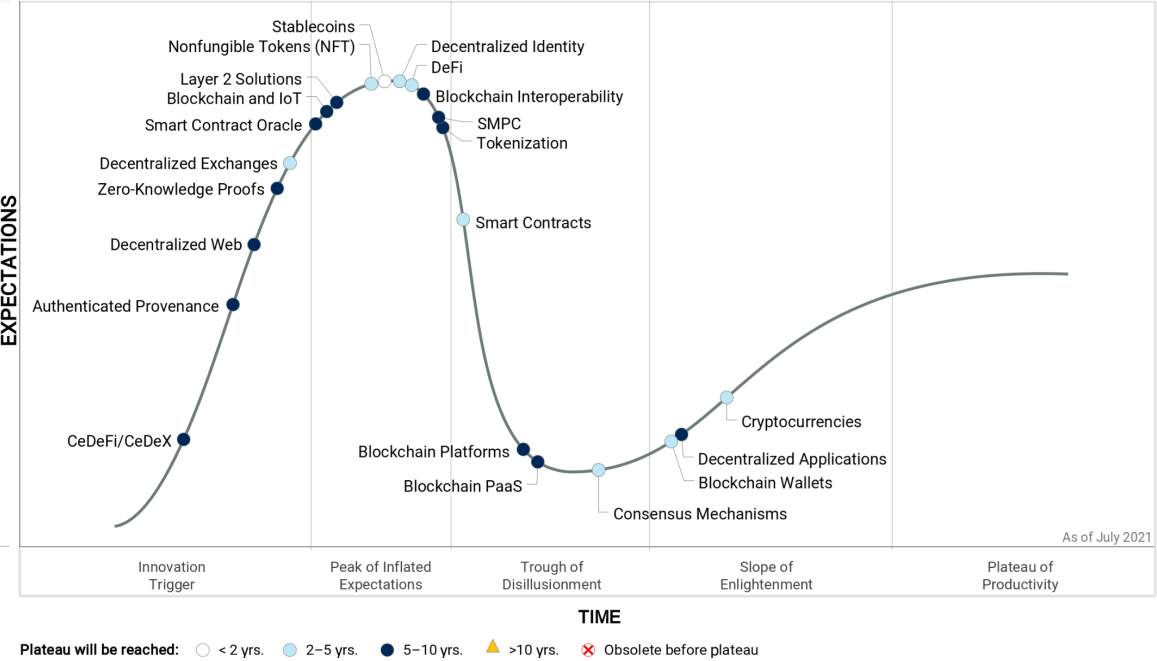
\includegraphics[width=\textwidth]{img/inleiding/gartner-hypecycle.png}
	\caption{\label{fig:gartner}Hype Cycle for Blockchain~\autocite{Gartner2021}}
\end{figure}

\pagebreak

In Figuur~\ref{fig:gartner} werd blockchain opgesplitst in 22 verschillende toepassingen. Elke toepassing werd voorgesteld als een punt op de Gartner Hype Cycle: een curve die weergeeft hoe de perceptie rond een hypetechnologie evolueert doorheen vijf vaste fases. Elk punt toont aan in welke fase de bijhorende toepassing zich bevindt (x-as) en als gevolg ook hoe hoog de verwachtingen errond zijn (y-as). De kleur van het punt stelt tevens een inschatting voor van hoe snel die toepassing matuur zal worden. 

Merk op dat 9 van de 22 toepassingen zich nog in de eerste opwaartse trend van de curve bevinden.
Die stijging wordt op gang getrokken door  een ``Innovation Trigger'' zoals een \textit{proof of concept} of belangstelling in de media. Men schat het potentieel heel hoog in, hoewel daar op dat moment nog weinig tot niets van in vervulling gebracht is. Hierdoor bereiken de verwachtingen al snel een maximum dat aanzienlijk hoger ligt dan wat de toepassing daadwerkelijk zal kunnen waarmaken: de ``Peak of Inflated Expectations''. Deze schromelijke overschatting zorgt gelukkig wel voor het nodige initiatief om de eerste commerciële projecten op poten te zetten. Een proces dat nog heel riskant is in dit ontwikkelingsstadium.

De ``Trough of Disillusionment'' maakt zijn intrede wanneer de eerste projecten niet het gewenste resultaat opleveren.
De verwachtingen van investeerders gaan de dieperik in door wat voor hen overkomt als mislukte experimenten. Desondanks is het een fase die zich aanbiedt als de geschikte gelegenheid tot onderzoek. Toepassingen, zoals ``Smart Contracts'' en ``Blockchain Platforms (aaS)'' komen stilaan \textit{down to earth} en vallen daarom mooi binnen de scope van deze paper. Een mix van succesverhalen en mislukkingen zorgen ervoor dat de grootste waanbeelden de deur uit zijn. De eerste commerciële implementaties doen hun intrede op de markt. Ze staan weliswaar nog in hun kinderschoenen, waardoor de vraag uit Sectie~\ref{sec:context} -- \nameref{sec:context} echt wel als een onderzoeksvraag mag beschouwd worden. 

In de huidige fase is het nog moeilijk om te beslissen of er mee op de trein gesprongen moet worden of niet. Met dit onderzoek kan hopelijk al een voorproefje gevonden worden van wat de ``Slope of Enlightenment'' zal brengen. Op die manier kan blockchain al benut worden voor de voordelen die binnen enkele jaren pas glashelder zullen worden. De ``Plateau of Productivity'' zal pas bereikt worden wanneer mainstream implementaties algemeen benut worden.

\newpage

\section{Opzet van deze bachelorproef}
\label{sec:opzet-van-deze-bachelorproef}

% Het is gebruikelijk aan het einde van de inleiding een overzicht te
% geven van de opbouw van de rest van de tekst. Deze sectie bevat al een aanzet
% die je kan aanvullen/aanpassen in functie van je eigen tekst.

De doelstelling van deze bachelorproef is om na te gaan of er een plaats is voor blockchain binnen het ERP-systeem van 14IT. Het is niet meteen duidelijk of het al dan niet haalbaar voor kmo's om data op te slaan in een blockchain. Daarnaast blijft ook nog de vraag of hier nuttige use cases voor weggelegd zijn. Om het onderzoek te laten slagen, was het van cruciaal belang om een resultaat na te streven dat praktisch bruikbaar is door 14IT. Dat gebeurde op twee manieren. 

Enerzijds moet dit werkstuk de lezer in staat stellen om zich op een vlotte manier in te werken in het onderwerp. Er valt al veel informatie te vinden over blockchains, waarvan niet even interessant is voor een ERP-systeem. De opbouw die in deze bachelorproef werd nagestreefd, zou 14IT moeten helpen om de state-of-the-art van het onderwerp snel te vatten.

Anderzijds biedt deze bachelorproef een \textit{proof of concept}. Deze zet de kennis en bevindingen van de sciptie om in een concrete toepassing. Het geeft 14IT een duidelijk beeld van wat mogelijk is binnen hun softwarepakket.


%%=============================================================================
%% Methodologie
%%=============================================================================

\chapter{Methodologie}
\label{ch:methodologie}

%% TODO: Hoe ben je te werk gegaan? Verdeel je onderzoek in grote fasen, en
%% licht in elke fase toe welke stappen je gevolgd hebt. Verantwoord waarom je
%% op deze manier te werk gegaan bent. Je moet kunnen aantonen dat je de best
%% mogelijke manier toegepast hebt om een antwoord te vinden op de
%% onderzoeksvraag.

Om de doelstelling van het onderzoek concreet te maken, werd volgende onderzoeksvraag geformuleerd:

\begin{center}
	\textit{\textbf{``Hoe kunnen softwareontwikkelaars overgaan tot integratie van blockchaintechnologie voor de dataopslag van hun ERP-systeem?''}}
\end{center}

Om op een systematische manier een antwoord te vinden op deze onderzoeksvraag, werd ze ontleed in vier deelvragen:

\begin{enumerate}
	\item Wat is een blockchain?
	\item Hoe wordt de data van het ERP-syteem opgeslagen? (\textit{as is})
	\item Welke mogelijkheden bieden blockchains voor een ERP-systeem?
	\item Hoe kunnen softwareontwikkelaars de data van hun ERP-systeem opslaan in een blockchain? (\textit{to be})
\end{enumerate}

Al van bij aanvang was het de bedoeling om, vertrekkende vanuit een high-level, zo snel mogelijk toe te werken naar de concrete bedrijfscasus. Die benadering weerspiegelt zich in de opgesomde deelvragen en de volgorde ervan.
Aan elk van de deelvragen werd een eigen hoofdstuk toegewijd.

Als eerste fase van het onderzoek, was het van cruciaal belang om een degelijk inzicht te verwerven in het onderwerp ``blockchain''. Dat gebeurde aan de hand van een \textbf{literatuurstudie} rond de eerste deelvraag van het onderzoek.
\textbf{Hoofdstuk~\ref{ch:blockchain} -- \nameref{ch:blockchain}} brengt de resultaten van deze studie samen, om de lezer zo de nodige achtergrond voor dit thema te bieden. Een rudimentaire implementatie van een blockchain wordt stap per stap opgebouwd, als oplossing voor een voorgedefiniëerde probleemstelling. Met deze opbouw komt de werking duidelijker naar voren. Dat is nodig om een gegrond inzicht te krijgen in de essentiële kenmerken van blockchains.

In \textbf{Hoofdstuk~\ref{ch:cpsolution} -- \nameref{ch:cpsolution}} werd het ERP-systeem van 14IT onder de loep genomen. Op die manier behandelt het de tweede deelvraag. Aan de hand van een \textbf{\textit{case study}} werd de huidige dataopslag van CPSolution in kaart gebracht. Daarmee werd het ``speelveld'' voor deze bachelorproef geconcretiseerd. Dat maakte het mogelijk om beter in te schatten welke noden, kansen en aandachtspunten er bestaan op vlak van dataopslag. Het was belangrijk om deze \textit{as-is} situatie voldoende te kennen, om zo gericht naar antwoorden op de volgende deelvraag te zoeken.

De voorgaande twee hoofdstukken leggen de basis voor de derde deelvraag. Deze wordt behandeld in \textbf{Hoofdstuk~\ref{ch:blockchaintoepassingen-voor-erp} -- \nameref{ch:blockchaintoepassingen-voor-erp}}. Aangezien zowel het begrip ``blockchain'' als ``ERP'' nu gekend is, kan gezocht worden naar een synergie tussen beide. Twee toepassingen uit de Gartner Hype Cycle\footnote{Zie Sectie~\ref{sec:verantwoording} -- \nameref{sec:verantwoording}.} geven de aanleiding tot NFT's, zo werd duidelijk uit een korte \textbf{literatuurverkenning}. Het kernidee dat tot de uiteindelijke \textit{proof of concept} leidde, is dat het mogelijk is om allerlei data in een blockchain op te nemen. Dat wordt geïllustreerd met een concreet voorbeeld van een NFT.

Een \textbf{\textit{proof of concept}} biedt het antwoord op de laatste deelvraag van het onderzoek. \textbf{Hoofdstuk~\ref{ch:proof-of-concept} -- \nameref{ch:proof-of-concept}} werd hieraan toegewijd. In dit hoofdstuk wordt een praktisch voorbeeld uitgewerkt van een blockchaintoepassing voor CPSolution. Hiervoor werd gesteund op de services van mintBlue, een bedrijf dat naar boven kwam bij een \textbf{marktverkenning} van het gekozen onderwerp.

Tenslotte, wordt in \textbf{Hoofdstuk~\ref{ch:conclusie} -- \nameref{ch:conclusie}} een antwoord geformuleerd op de overkoepelende onderzoeksvraag. 



% Voeg hier je eigen hoofdstukken toe die de ``corpus'' van je bachelorproef
% vormen. De structuur en titels hangen af van je eigen onderzoek. Je kan bv.
% elke fase in je onderzoek in een apart hoofdstuk bespreken.

\chapter{Blockchain}
\label{ch:blockchain}

% Tip: Begin elk hoofdstuk met een paragraaf inleiding die beschrijft hoe
% dit hoofdstuk past binnen het geheel van de bachelorproef. Geef in het
% bijzonder aan wat de link is met het vorige en volgende hoofdstuk.

Dit hoofdstuk is het resultaat van een literatuurstudie, toegespitst op de eerste deelvraag van het onderzoek:

\begin{center}
	\textit{\textbf{``Wat is een blockchain?''}}
\end{center}

Vertrekkende vanuit het \textit{double-spendingprobleem}, wordt geïllustreerd dat het delen van een grootboek \textit{of ledger} onvermijdelijk voor vertrouwenskwesties zorgt. Dit issue werd voor geruime tijd enkel vanuit een gecentraliseerd systeem benaderd. Met het verlangen naar de eerste \textit{cryptocurrencies} ontstond de nood aan een gedecentraliseerde benadering. Een blockchain vormde de oplossing voor de problemen die daarbij kwamen opdagen.

Volgende secties werden opgebouwd met als doel een inzicht te geven in de structuur van een blockchain en hoe zijn structuur tot stand kwam. Daarom wordt vertrokken vanuit een veralgemeende probleemstelling. Door deze \textit{case} stelselmatig aan te vullen met enkele basisprincipes komen we uiteinlijk tot een oplossing onder de vorm van een blockchain. Voor de uitwerking hiervan werd de implementatie van de eerste blockchain, zoals bedacht door Nakamoto, gebruikt als boegbeeld. Op die manier toont dit hoofdstuk hoe een blockchain aan zijn eigenschappen komt. Wie deze in het achterhoofd houdt, zal met een gefundeerd begrip de volgende deelvragen kunnen aanvatten.

% Pas na deze inleidende paragraaf komt de eerste sectiehoofding.


\section{Gedeelde ledgers}
\label{sec:gedeelde-ledgers}
In de whitepaper ``Bitcoin: A Peer-to-Peer Electronic Cash System'' werkte Satoshi Nakamoto het voorstel uit van wat men vandaag een blockchain noemt. Met een vernuftige keten van datablokken loste Nakamoto het zogenaamde \textit{double-spendingprobleem} op. Het \textit{incentive} was om Bitcoin, de eerste gedecentraliseerde cryptomunt, uit te brengen. Voor dit onderzoek is het echter zinvol om de context zo min mogelijk vast te hangen aan \textit{cryptocurrencies}. Daarom zullen we het begrip ``transacties'' ook opentrekken naar andere toepassingsgebieden. Een veralgemeende probleemstelling rond zogenaamde \textit{ledgers} zal het vertrekpunt vormen van een meer technische uiteenzetting.


\subsection{Double-spending}
\label{sub:double-spending}

Double-spending is een probleem binnen de context van \textit{cryptocurrencies}. Het doet zich voor wanneer een partij eenzelfde digitale token voor meerdere transacties gebruikt, hoewel dit maar voor een het geval zou mogen zijn~\autocite{Chohan2021}. Digitale munten kunnen namelijk (net zoals fysiek geld) gedupliceerd of vervalst worden. In tegenstelling tot tastbaar geld, bestaan digitale munten echter uitsluitend uit binaire data. Dat maakt de strijd tegen vervalsing extra uitdagend. Een kenteken van authenticiteit toevoegen, is op het eerste zicht niet mogelijk. Data kan namelijk heel gemakkelijk gerepliceerd worden. Een simpele aanduiding, analoog aan de zilverstrook op een bankbiljet, is bij een cryptomunt dus compleet zinloos. Het zou met een eenvoudige copy-paste kunnen vervalst worden~\autocite{Hoepman2008}. Om cryptomunten op de markt te brengen, waren dus andere oplossingen nodig.


\subsection{Transacties}
\label{sub:transacties}

Een transactie staat voor een interaction tussen partijen~\autocite{Salem2008}. In de oorspronkelijke toepassing van blockchains betekende dit de bitcoin-overdracht van een partij naar een andere~\autocite{Pierro2017}. Er zijn echter veel meer transacties denkbaar dan enkel eenvoudige gelduitwisselingen.
In het boek ``Blockchain: Blueprint for a New Economy'' wordt blockchain-technologie opgedeeld in drie fases. De bijhorende toepassingsgebieden bepalen de transacties die denkbaar zijn om op te nemen in een blockchain~\autocite{Swan2015}.

\textbf{Blockchain 1.0} is het label voor blockchain-technologie, zoals die bestond in zijn oorspronkelijke context: cryptocurrencies. Een transactie staat in die context voor
\begin{itemize}
	\item het spenderen van een cryptomunt.
\end{itemize}
\textbf{Blockchain 2.0} staat voor een uitbreiding van de technologie, die voornamelijk beperkt blijft tot de financiële sector. Banken, betalingen en de \textit{supply chain} geven aanleiding tot transacties zoals
\begin{itemize}
	\item afsluiten van \textit{smart contracts}
	\item uitwisselen van aandelen;
	\item uitwisselen van hypotheken;
	\item afsluiten van een abonnement;
	\item afsluiten van een verzekering;
	\item het versturen van een digitale factuur;
	\item ...
\end{itemize}
\textbf{Blockchain 3.0} wordt beschreven als de toepassing van blockchain in sectoren zoals gezondheidszorg, wetenschap, cultuur en de overheid~\autocite{Xu2019}. De uitwisseling die dan plaatsvindt gaat niet zozeer over financiële zaken, maar over informatie die ontstaat bij
\begin{itemize}
	\item de waarnemingen van een metaaldetector bij voedingsproductie;
	\item het toedienen van een inenting;
	\item het indienen van een subsidieaanvraag bij de overheid;
	\item ...
\end{itemize}

Ook al deze zaken horen uiteraard onvervalsbaar te zijn. Door het begrip transactie ruimer te bekijken, kan double-spending vertaald worden naar veralgemeende probleemstelling. Dit is zinvol, aangezien de \textit{use cases} voor dit onderzoek niet te vinden zijn in Blockchain 1.0, maar starten bij Blockchain 2.0.


\subsection{Probleemstelling}
\label{sub:probleemstelling}

In de gegeven context kunnen drie partijen onderlinge transacties uitvoeren. Er ontstaat nood aan een gedeeld grootboek of \textit{ledger} om al deze transacties in op te nemen. In deze ledger moet elke partij
\begin{itemize}
	\item nieuw uitgevoerde transacties kunnen opslaan;
	\item de voorgaande transacties kunnen raadplegen.
\end{itemize}

De ledger moet uiteraard betrouwbaar zijn. Dit wil zeggen dat er geen vervalste of gedupliceerde regels mogen voorkomen in de ledger.

\begin{figure}[H]
	\centering
	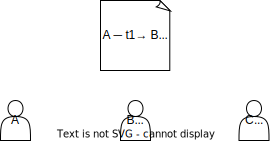
\includegraphics[]{img/blockchain/probleemstelling.pdf}
	\caption{\label{fig:probleemstelling}Probleemstelling}
\end{figure}

\begin{tcolorbox}[title=Voorbeeld]	
Partij A voert een transactie uit met partij B. Partij A schrijft de transactie weg in de ledger.

Partij C voert een transactie uit met partij A. Partij C schrijft de transactie weg in de ledger.
\end{tcolorbox}

Er schuilt een inherente vertrouwenskwestie in het bijhouden van een gedeelde ledger: alle deelnemedende partijen moeten elkaar vertrouwen. Volgende kwestie lijkt op het double-spendingprobleem bij cryptomunten:

\textbf{Probleem:} 
Partij A voert geen transactie uit met partij B, maar schrijft toch een lijn weg in de ledger. Partij B gaat hier uiteraard niet mee akkoord. Voor partij C lijkt het alsof er nog een transactie plaatsvond tussen A en B.


\subsection{Centralized ledger}
\label{sub:centralized-ledger}

Voorgaande probleemstelling werd traditioneel aangepakt vanuit een gecentraliseerd systeem. Er wordt een onafhankelijke partij ingeschakeld voor het bijhouden en bewaken van de ledger~\autocite{Rawat2020}. Deze derde partij houdt de ledger bij op een centrale databank die raadpleegbaar is door alle andere partijen. Wie een transactie wilt wegschrijven in de ledger, doet een aanvraag die kan gecheckt worden. Op die manier waakt de centrale partij erover dat er enkel geldige en geverifieerde transacties in de ledger kunnen komen. 

Om te authenticiteit van een transactie aan te tonen wordt in de praktijk gebruik gemaakt van een \textit{digital signature}~\autocite{Salem2008}. Het vormt de oplossing voor het \textit{copy-pasteprobleem} dat werd aangehaald in subsectie \ref{sub:double-spending} - \nameref{sub:double-spending}. Door bij elke regel een unieke code te gegenereren op basis van een publieke en private sleutel, kan deze later geverifiëerd worden\footnote{Een diepgaandere uiteenzetting van \textit{digital signatures} is in dit onderzoek niet aan de orde.}. Net zoals een handtekening bij fysieke documenten, wordt zo de probleemstelling aangepakt.

\begin{figure}[H]
	\centering
	\includegraphics[]{img/blockchain/centralized-ledger.pdf}
	\caption{\label{fig:centralized-ledger}Centralized ledger}
\end{figure}

Merk op dat de probleemstelling in principe niet volledig opgelost is. De vertrouwenskwestie die partijen onderling hadden, is in zekere zin gewoon verschoven naar het nieuwe, centrale figuur. Dit kan gezien worden als een Single Point of Failure~\autocite{Majaski2021}.

\textbf{Probleem:} 
Op vraag van partij A verwijdert het centrale figuur een voorgaande transactie tussen A en B. 
Aangezien dit de enige kopie is van de ledger is er geen manier voor partij B om hierop terug te komen. Parij C weet niets over het hele scenario.

Met een gedistribueerd systeem kan men de nood aan een centrale authoriteit proberen vermijden.


\subsection{Distributed ledger}
\label{sub:distributed-ledger}

Om de nood aan een centrale opslagplaatst te omzeilen, zou elke partij een eigen kopie kunnen bijhouden van de gezamenlijke ledger. Zo kan elke partij over zijn kopie waken en valse transacties onderscheppen. Om een nieuwe regel toe te voegen aan de ledger, wordt een signaal \textit{gebroadcast} op het netwerk. De ontvangende partijen kunnen hierna hun versie van de ledger updaten~\autocite{Nakamoto2008}. Hierdoor ontstaat echter een nieuw probleem.

\begin{figure}[H]
	\centering
	\includegraphics[]{img/blockchain/distributed-ledger.pdf}
	\caption{\label{fig:distributed-ledger}Distributed ledger}
\end{figure}

\textbf{Probleem:} Partij A voert een transactie uit met partij B, maar broadcast dit niet naar partij C. De ledger van partij C stemt niet meer overeen met die van A en B.

Hoewel het handig is dat elke partij zijn eigen versie van de gedeelde ledger heeft, laat dit een nieuwe vraag ontstaan: wat is ``de juiste'' versie? Om transacties correct bij te houden in een gedistribueerd systeem, is er nood aan een protocol, een technologie die deelnemende partijen een manier biedt om het eens te zijn over wat de correcte ledger is. Die technologie staat bekend als een blockchain~\autocite{Chaudhry2018}.


\section{Uitgangspunten}
\label{sec:uitgangspunten}

De blockchain kwam als oplossing voor het probleem dat beschreven wordt in subsectie \ref{sub:distributed-ledger} - \nameref{sub:distributed-ledger}. Zoals reeds aangegeven, werd dit probleem voor het eerst opgelost bij de ontwikkeling van de Bitcoin. Om een gegrond inzicht te geven in de eigenschappen van een blockchain, is deze sectie opgedeeld in drie basisprincipes. De concrete invulling van die principes is gebaseerd op de oorspronkelijke implementatie door Nakamoto.

Volgende subsecties zullen aantonen hoe het vertrouwensprobleem bij een \textit{distributed ledger} kan opgelost worden door het gezamenlijk opstellen van een keten van datablokken: een proces genaamd mining.


\subsection{Blokken}
\label{sub:blokken}

Een eerste basisprincipe is dat de ledger wordt opgebouwd uit zogenaamde blokken die elk een apart deel van de transacties oplijsten. Deze blokken worden om de zoveel tijd gegenereerd door een proces dat ``mining'' genoemd wordt~\autocite{Bhaskar2015}.

Tijdens het minen, wordt gedurende een beperkte tijdsspanne geluisterd naar de transacties die gebroadcast worden over het netwerk. Het blok houdt deze transacties dan bij onder de vorm van een Merkle Tree\footnote{Deze speciale binaire boom maakt handig gebruik van hashing om de transacties van het blok snel valideerbaar te maken. Deze datastructuur wordt uitsluitend gebruikt binnen een blok. Om verwarring te vermijden met de structuur van de blockchain als geheel, wordt deze verder niet besproken.}~\autocite{Salem2008}. Op die manier omvat het een uniek deel van de ledger. Wanneer de tijdslimiet verstreken is, kan de opbouw van het blok afgerond worden~\autocite{Nakamoto2008}. Hierbij gebeuren nog een aantal essentiële stappen die in de volgende subsecties besproken worden. 

Wanneer een blok klaar is, wordt het in zijn geheel \textit{gebroadcast}, waarna het door de deelnemers van het netwerk kan geaccepteerd worden~\autocite{Nakamoto2008}. Zo wordt de distributed ledger stuk per stuk aangevuld.
Om deze stukken aan elkaar te linken, zal elk blok ook een verwijzing krijgen naar zijn voorganger. Voor deze verwijzing wordt gebruik gemaakt van een cryptografische hashfunctie. 

\begin{figure}[H]
	\centering
	\includegraphics[]{img/blockchain/blokken.pdf}
	\caption{\label{fig:blokken}Gedeelde ledger, opgedeeld in blokken}
\end{figure}

\subsection{Cryptohashes}
\label{sub:cryptohashes}

Naast een lijst van transacties, houdt elk blok ook een verwijzing bij naar het voorgaande blok. Deze verwijzing is onder de vorm van een hashwaarde die bepaald wordt door een hashfunctie zoals SHA-256~\autocite{Nakamoto2008}. Wanneer die functie een blok als input krijgt, geeft deze een binaire tekenreeks van vaste lengte als output~\autocite{Slaats2019}. Die tekenreeks wordt dan gebruikt als verwijzing naar het voorgaande blok. Op die manier komt men tot een keten van blokken: een blockchain.

\begin{center}
	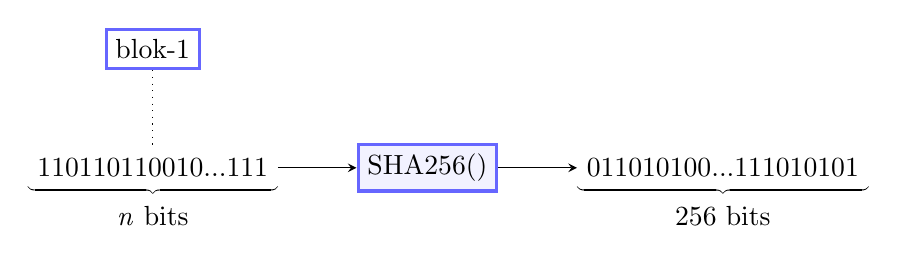
\begin{tikzpicture}[
		roundnode/.style={circle, draw=green!60, fill=green!5, very thick, minimum size=7mm},
		squarednode/.style={rectangle, draw=blue!60, fill=blue!5, very thick, minimum size=5mm},
		]
		%Nodes
		\node[squarednode,fill=none]  (blok-1)        					    {blok-1};
		\node[draw=none,fill=none]    (input)         [below=of blok-1]       {110110110010...111};
		\node[draw=none,fill=none]    (output-length) [below=of input, yshift=25]		{\textit{n} bits};
		\node[squarednode]            (sha256) 		  [right=of input]       {SHA256()};
		\node[draw=none,fill=none]    (output)        [right=of sha256]		{011010100...111010101};
		\node[draw=none,fill=none]    (output-length) [below=of output, yshift=25]		{256 bits};
		
		% Calligraphic brace
		\draw [decorate, decoration = {calligraphic brace}] (input.south east) --  (input.south west);
		\draw [decorate, decoration = {calligraphic brace}] (output.south east) --  (output.south west);
		
		%Lines
		\draw[dotted] (blok-1.south) -- (input.north);
		\draw[-stealth] (input.east) -- (sha256.west);
		\draw[-stealth] (sha256.east) -- (output.west);
		
	\end{tikzpicture}
\end{center}

Voor elke input van de hashfunctie, kan eenvoudig de output bepaald worden. Toch is het geheel onwezenlijk om de inverse berekening te maken. Daarom wordt deze hashfunctie cryptografisch genoemd. Dit is een van de sleutelkenmerken die blockchain mogelijk maken: het is niet haalbaar om de input van een gegeven hashwaarde te \textit{reverse-engineeren}~\autocite{Mansfield2018}. 

Het is belangrijk om erop te wijzen dat zelfs de kleinste wijziging aan de input van een hashfunctie, een drastisch verschil maakt aan de output. In deze context betekent dit dat een wijziging aan een blok (hoe klein dan ook) ervoor zorgt dat zijn hashwaarde volledig verandert. Aangezien deze hashwaarden gebruikt worden om de blokken aan elkaar te ketenen, zal de blockchain hierdoor ergens doorbroken worden. De hashwaarde die naar dit blok verwees is namelijk niet meer correct.~\autocite{Salem2008} Om terug tot een geldige blockchain te komen zal er een hele kettingreactie moeten plaatsvinden. Onderstaand voorbeeld illustreert waarom dit het geval is:

\begin{tcolorbox}[title=Voorbeeld]	
	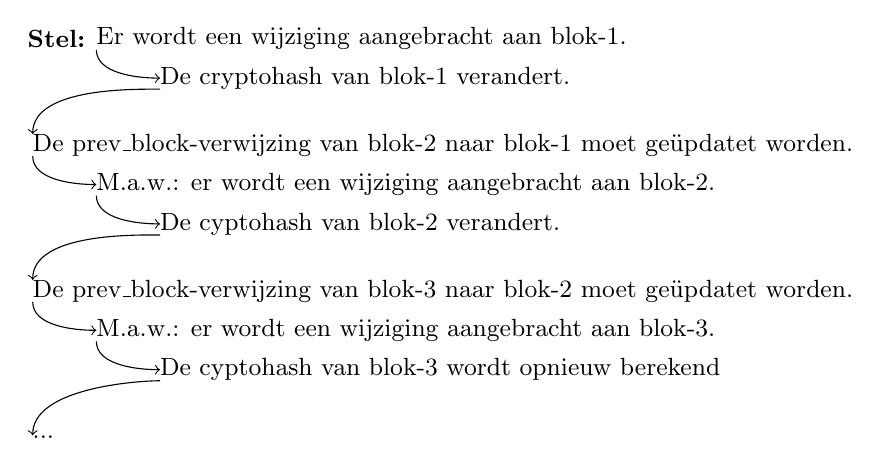
\begin{tikzpicture}[every node/.style={inner sep=0,outer sep=0, font=\small}, align=left, node distance=.5]
		
		%Nodes
		\node[draw=none,fill=none] (11)        					    {\textbf{Stel: }};
		\node[draw=none,fill=none] (12) [right=of 11, xshift=-15] {Er wordt een wijziging aangebracht aan blok-1.};
		\node[draw=none,fill=none] (13) [below=of 12.west, anchor=west, xshift=23] {De cryptohash van blok-1 verandert.};
		\node[draw=none,fill=none] (21) [below=of 13.west, anchor=west, xshift=-46, yshift=-10]  {De prev\_block-verwijzing van blok-2 naar blok-1 moet geüpdatet worden.};
		\node[draw=none,fill=none] (22) [below=of 21.west, anchor=west, xshift=23]  {M.a.w.: er wordt een wijziging aangebracht aan blok-2.};
		\node[draw=none,fill=none] (23) [below=of 22.west, anchor=west, xshift=23]  {De cyptohash van blok-2 verandert.};
		\node[draw=none,fill=none] (31) [below=of 23.west, anchor=west, xshift=-46, yshift=-10]  {De prev\_block-verwijzing van blok-3 naar blok-2 moet geüpdatet worden.};
		\node[draw=none,fill=none] (32) [below=of 31.west, anchor=west, xshift=23]  {M.a.w.: er wordt een wijziging aangebracht aan blok-3.};
		\node[draw=none,fill=none] (33) [below=of 32.west, anchor=west, xshift=23]  {De cyptohash van blok-3 wordt opnieuw berekend};
		\node[draw=none,fill=none] (41) [below=of 33.west, anchor=west, xshift=-46, yshift=-10]  {...};
		
		%Lines
		\draw[->] (12.south west) .. controls +(down:3mm) and +(left:3mm) .. (13.west);
		\draw[->] (13.south west) .. controls +(left:3mm) and +(up:6mm) .. (21.north west);
		\draw[->] (21.south west) .. controls +(down:3mm) and +(left:3mm) .. (22.west);
		\draw[->] (22.south west) .. controls +(down:3mm) and +(left:3mm) .. (23.west);
		\draw[->] (23.south west) .. controls +(left:3mm) and +(up:6mm) .. (31.north west);
		\draw[->] (31.south west) .. controls +(down:3mm) and +(left:3mm) .. (32.west);
		\draw[->] (32.south west) .. controls +(down:3mm) and +(left:3mm) .. (33.west);
		\draw[->] (33.south west) .. controls +(left:3mm) and +(up:6mm) .. (41.north west);
	\end{tikzpicture}	
\end{tcolorbox}

Bovenstaand voorbeeld toont aan dat de inhoud van een blok niet gewijzigd kan worden, zonder ook alle daaropvolgende blokken te wijzigen. Het gaat namelijk steeds gepaard met de wijziging van de bijhorende hash. Aangezien deze hash altijd deel uitmaakt van een daaropvolgend blok, zullen al deze verwijzingen moeten herberekend worden~\autocite{Nakamoto2008}.

Niemand zal nog een aanpassing kunnen maken aan de ledger zoals:
\begin{itemize}
	\item een transactie wijzigen, toegevoegen of verwijderen;
	\item het verwisselen van transacties;
	\item het verwisselen van blokken;
\end{itemize}

zonder verantwoordelijk te worden voor alle hashverwijzingen na het geïmpacteerde punt. Op die manier wordt al een eerste stap gezet naar een onvervalsbare, of \textit{immutable} \textit{distributed ledger}. Het doel is echter nog niet bereikt.

\textbf{Probleem:} 
Wie de ledger wenst te vervalsen hoeft zich geen zorgen te maken over het doorbreken van de keten. 
Door simpelweg de nodige hashes opnieuw te berekenen, komt men uiteindelijk terug tot een geldige blockchain. Dat kan, aangezien uitvoeren van een hashfunctie in constante tijd kan gebeuren~\autocite{Slaats2019}. Op die manier kunnen nog steeds tegenstrijdige, maar technisch geldige ledgers ontstaan.

Een laatste essentieel principe bestaat eruit om bij elk blok een extra speciaal stuk data te eisen, waardoor het vinden van een gepaste hash wel een rekenintesieve opdracht wordt. Op die manier wordt ook het bovenstaande probleem opgelost.

\begin{figure}[H]
	\centering
	\includegraphics[]{img/blockchain/blokken-met-cryptohash.pdf}
	\caption{\label{fig:blokken-met-cryptohash}Blokken met een cryptohash als verwijzing}
\end{figure}

\subsection{Proof of Work}
\label{sub:proof-of-work}

De laatste sleutel bestaat eruit om een extra stukje data toe te voegen aan elk blok genaamd de ``Proof of Work''.
Afhankelijk van de inhoud van die Proof of Work, zal het blok uiteraard veranderen, en als gevolg ook de hash van dat blok~\autocite{Nakamoto2008}. Met andere woorden: door dit stukje data te tweaken, wijzigt men de hash die nodig is om te verwijzen naar dat blok.

Het opzet is om nu een extra vereiste op te leggen aan die hashverwijzingen, zodat het tijdrovend wordt om die PoW te produceren. Nakamoto vond een dergelijke vereiste, die desondanks eenvoudig is om te verifiëren: de has moet beginnen met een voorgedefiniëerd aantal nul-bits. Een blok zal pas als geldig beschouwd worden, wanneer de eerste \textit{x} bits allemaal de waarde nul hebben. 

\begin{center}
	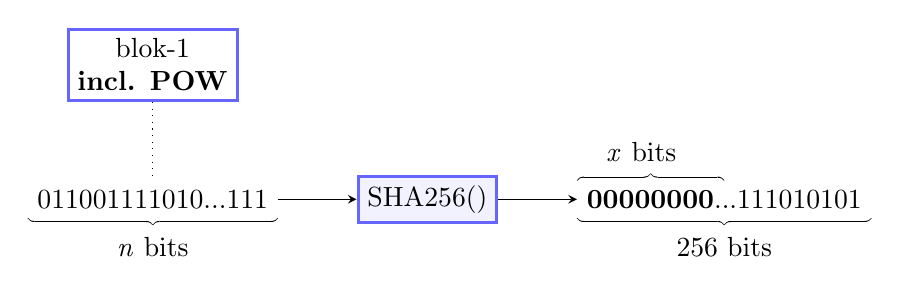
\begin{tikzpicture}[
		roundnode/.style={circle, draw=green!60, fill=green!5, very thick, minimum size=7mm},
		squarednode/.style={rectangle, draw=blue!60, fill=blue!5, very thick, minimum size=5mm},
		]
		%Nodes
		\node[squarednode,fill=none, align=center]  (blok-1)        					    {blok-1\\\textbf{incl. POW}};
		\node[draw=none,fill=none]    (input)         [below=of blok-1]       {011001111010...111};
		\node[draw=none,fill=none]    (output-length) [below=of input, yshift=25]		{\textit{n} bits};
		\node[squarednode]            (sha256) 		  [right=of input]       {SHA256()};
		\node[draw=none,fill=none]    (output)        [right=of sha256]		{\textbf{00000000}...111010101};
		\node[draw=none,fill=none]    (output-length) [above=of output, xshift=-30, yshift=-25]		{\textit{x} bits};
		\node[draw=none,fill=none]    (output-length) [below=of output, yshift=25]		{256 bits};
		
		% Calligraphic brace
		\draw [decorate, decoration = {calligraphic brace}] (input.south east) --  (input.south west);
		\draw [decorate, decoration = {calligraphic brace}] (output.north west) --  (output.north);
		\draw [decorate, decoration = {calligraphic brace}] (output.south east) --  (output.south west);
		
		%Lines
		\draw[dotted] (blok-1.south) -- (input.north);
		\draw[-stealth] (input.east) -- (sha256.west);
		\draw[-stealth] (sha256.east) -- (output.west);
	\end{tikzpicture}
\end{center}

Om tot een geldig blok te komen, zal dus telkens een PoW-waarde gezocht moeten worden, die de hash van dat blok laat starten met de nodige nulbits. Aangezien het hier over een cryptografische hasahfunctie gaat, valt die Proof of Work niet zomaar te voorspellen~\autocite{Mansfield2018}. Er zit niets anders op dan herhaaldelijk willekeurige waarden uit te proberen, tot er toevallig een geldige hashwaarde uit voortkomt.

\begin{flushright}
	\textit{{\small ``The proof-of-work involves scanning for a value that when hashed, such as with SHA-256, the hash begins with a number of zero bits. The average work required is exponential in the number of zero bits required and can be verified by executing a single hash.''}}
	
	~\autocite{Nakamoto2008}
\end{flushright}

Onderstaand voorbeeld illustreert hoe de kettingreactie bij het wijzigen van een blok er nu uitziet:

\begin{tcolorbox}[title=Voorbeeld]	
	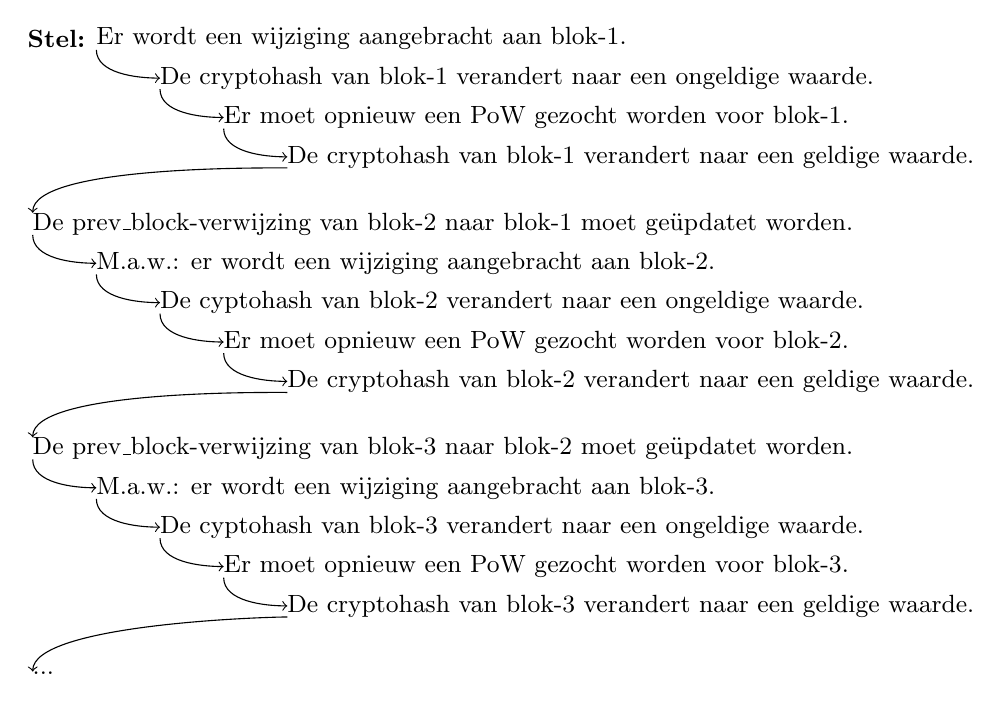
\begin{tikzpicture}[every node/.style={inner sep=0,outer sep=0, font=\small}, align=left, node distance=.5]
		
		%Nodes
		\node[draw=none,fill=none] (11)        					    {\textbf{Stel: }};
		\node[draw=none,fill=none] (12) [right=of 11, xshift=-15] {Er wordt een wijziging aangebracht aan blok-1.};
		\node[draw=none,fill=none] (13) [below=of 12.west, anchor=west, xshift=23] {De cryptohash van blok-1 verandert naar een ongeldige waarde.};
		\node[draw=none,fill=none] (14) [below=of 13.west, anchor=west, xshift=23] {Er moet opnieuw een PoW gezocht worden voor blok-1.};
		\node[draw=none,fill=none] (15) [below=of 14.west, anchor=west, xshift=23] {De cryptohash van blok-1 verandert naar een geldige waarde.};
		\node[draw=none,fill=none] (21) [below=of 15.west, anchor=west, xshift=-92, yshift=-10]  {De prev\_block-verwijzing van blok-2 naar blok-1 moet geüpdatet worden.};
		\node[draw=none,fill=none] (22) [below=of 21.west, anchor=west, xshift=23]  {M.a.w.: er wordt een wijziging aangebracht aan blok-2.};
		\node[draw=none,fill=none] (23) [below=of 22.west, anchor=west, xshift=23]  {De cyptohash van blok-2 verandert naar een ongeldige waarde.};
		\node[draw=none,fill=none] (24) [below=of 23.west, anchor=west, xshift=23] {Er moet opnieuw een PoW gezocht worden voor blok-2.};
		\node[draw=none,fill=none] (25) [below=of 24.west, anchor=west, xshift=23] {De cryptohash van blok-2 verandert naar een geldige waarde.};
		\node[draw=none,fill=none] (31) [below=of 25.west, anchor=west, xshift=-92, yshift=-10]  {De prev\_block-verwijzing van blok-3 naar blok-2 moet geüpdatet worden.};
		\node[draw=none,fill=none] (32) [below=of 31.west, anchor=west, xshift=23]  {M.a.w.: er wordt een wijziging aangebracht aan blok-3.};
		\node[draw=none,fill=none] (33) [below=of 32.west, anchor=west, xshift=23]  {De cyptohash van blok-3 verandert  naar een ongeldige waarde.};
		\node[draw=none,fill=none] (34) [below=of 33.west, anchor=west, xshift=23] {Er moet opnieuw een PoW gezocht worden voor blok-3.};
		\node[draw=none,fill=none] (35) [below=of 34.west, anchor=west, xshift=23] {De cryptohash van blok-3 verandert naar een geldige waarde.};
		\node[draw=none,fill=none] (41) [below=of 35.west, anchor=west, xshift=-92, yshift=-10]  {...};
		
		%Lines
		\draw[->] (12.south west) .. controls +(down:3mm) and +(left:3mm) .. (13.west);
		\draw[->] (13.south west) .. controls +(down:3mm) and +(left:3mm) .. (14.west);
		\draw[->] (14.south west) .. controls +(down:3mm) and +(left:3mm) .. (15.west);
		\draw[->] (15.south west) .. controls +(left:3mm) and +(up:6mm) .. (21.north west);
		\draw[->] (21.south west) .. controls +(down:3mm) and +(left:3mm) .. (22.west);
		\draw[->] (22.south west) .. controls +(down:3mm) and +(left:3mm) .. (23.west);
		\draw[->] (23.south west) .. controls +(down:3mm) and +(left:3mm) .. (24.west);
		\draw[->] (24.south west) .. controls +(down:3mm) and +(left:3mm) .. (25.west);
		\draw[->] (25.south west) .. controls +(left:3mm) and +(up:6mm) .. (31.north west);
		\draw[->] (31.south west) .. controls +(down:3mm) and +(left:3mm) .. (32.west);
		\draw[->] (32.south west) .. controls +(down:3mm) and +(left:3mm) .. (33.west);
		\draw[->] (33.south west) .. controls +(down:3mm) and +(left:3mm) .. (34.west);
		\draw[->] (34.south west) .. controls +(down:3mm) and +(left:3mm) .. (35.west);
		\draw[->] (35.south west) .. controls +(left:3mm) and +(up:6mm) .. (41.north west);
	\end{tikzpicture}	
\end{tcolorbox}


Een wijziging aan een blok zorgt er dus nog steeds voor dat alle daaropvolgende hashes herevalueerd moeten worden. Door de toevoeging van de PoW is die herevaluatie nu ook een rekenintesieve opdracht geworden. Om een verwijzing te herstellen moet namelijk steeds opnieuw een geldige hashwaarde gevonden worden. Om die te vinden moet gescand worden naar een gepaste PoW-waarde.

\begin{figure}[H]
	\centering
	\includegraphics[]{img/blockchain/blokken-met-pow.pdf}
	\caption{\label{fig:blokken-met-pow}Proof of Work als onderdeel van de blokken.}
\end{figure}


\section{Essentiële principes}
\label{sec:eigenschappen}

Blockchains bieden dus een techniek om transacties zodanig bij te houden dat deze later niet meer vervalst kunnen worden.
De essentie van de technologie die door voorgaande secties tot stand komt, kan beschreven worden vanuit enkele (Engelstalige) basisprincipes.

\subsection{Decentralization}
\label{sub:decentralization}

Er bestaat geen centrale authoriteit over de ledger die wordt bijgehouden in een blockchain. Het wordt mogelijk gemaakt door verschillende partijen of nodes die samenwerken in een netwerk~\autocite{Anita2019}.

\subsection{Peer-to-peer network}
\label{sub:peer-to-peer-network}

In het netwerk is elke node instaat om overdrachten van transacties en blokken te starten en te beëindigen. Dat maakt het een peer-to-peernetwerk.~\autocite{Davidson2016} Hierin worden voortdurend volgende stappen doorlopen~\autocite{Nakamoto2008}:

\begin{enumerate}
	\item Nieuwe transacties worden naar alle nodes van het netwerk gebroadcast.
	\item Elke node verzamelt deze nieuwe transactions in een blok.
	\item Elke node zoekt naar een Proof of Work voor zijn blok.
	\item Eens een Proof of Work gevonden is, wordt het blok in zijn geheel naar alle andere nodes gebroadcast.
	\item Nodes aanvaarden het blok als alle transactions geldig zijn.
	\item Nodes ``accepteren'' een blok door zijn hash te gebruiken als verwijzing in het volgende blok.
\end{enumerate}

\subsection{Consensus}
\label{sub:consensus}

Nodes zullen vervolgens altijd de langste keten van blokken beschouwen als de correcte versie van de ledger. De idee is namelijk dat de ``eerlijke'' blockchain degene is die het snelste groeit, aangezien dit de versie is waarvoor de meeste nodes naar Proof of Work's zoeken. Daardoor kan elke partij een consensus vormen over wat de correcte versie van de ledger is~\autocite{Anita2019}.

\subsection{Incorruptibility}
\label{sub:incorruptibility}

Het is belangrijk om erop te wijzen dat het in principe niet onmogelijk om een blockchain aan te passen. Het is wel nagenoeg onmogelijk om als minderheid de rest van het netwerk te overtuigen dat die versie van de ledger de correcte is. Daarvoor zou men namelijk de langste blokketen moeten produceren. Dat houdt in dat er voortdurend naar de Proof of Work van nieuwe blokken moet gezocht worden. In die - rekenintensieve - opdracht, zal de ``bedriegende'' minderheid uiteindelijk altijd het onderspit moeten delven voor de ``eerlijke'' meerderheid. Daarom verkiest men het soms om een blockchain als \textit{incorruptible} te beschrijven, in plaats van \textit{immutable}~\autocite{Salem2008}.

Ook bij deze \textit{incorruptibility} valt echter een kanttekening te maken. Het syteem is maar veilig, voor zolang de eerlijke nodes gezamenlijk over meer CPU-kracht beschikken dan eender welke groep aanvallende nodes~\autocite{Nakamoto2008}. Indien de aanvallende nodes samen het gros van de CPU-kracht beheersen, kunnen deze wel de blockchain trachten te corrumperen\footnote{Dergelijke aanvallen hebben al plaatsgevonden, voornamelijk bij kleinschalige cryptomunten. Ze werden dan het slachtoffer van wat men een ``51 percent attack'' noemt. Om dit te verhinderen werden al protocollen bedacht die buiten de scope van dit onderzoek vallen.}~\autocite{Anita2019}.



\chapter{ERP as is}
\label{ch:blockchain}
\chapter{Blockchain for ERP}
\label{ch:blockchain-for-erp}

In dit hoofdstuk wordt de derde deelvraag van het onderzoek behandeld:

\begin{center}
	\textit{\textbf{``Welke mogelijkheden biedt blockchain voor een ERP-systeem?''}}
\end{center}


\section{Blockchain-platformen}

De originele Bitcoin whitepaper inspireerde talloze spelers om een eigen versie van een blokchain te ontwikkelen. Ondertussen brachten al verschillende ondernemingen hun eigen variant op de markt. Om deze implementaties van elkaar te onderscheiden spreekt men over verschillende ``blockchain-platformen''. Elk platform biedt een basis aan ontwikkelaars om nieuwe toepassingen te bouwen op de bestaande blokchain-infrastructuur
~\autocite{Saraf2018}.

\begin{table}[H]
	\begin{tabular}{@{}lccc@{}}
		\cmidrule(l){2-4}
		& \textbf{Ethereum}                                         & \textbf{Hyperledger} & \textbf{R3 Corda}                                        \\ \midrule
		1. Type                                                                     & Openbaar                                                  & Besloten             & Besloten                                                 \\ \midrule
		2. Consensus algoritme                                                      & Proof of Work                                             & Pluggable Framework  & Pluggable Framework                                      \\ \midrule
		3. Toepassingsgebied                                                        & Algemeen                                                  & Algemeen             & Financiële sector                                        \\ \midrule
		\begin{tabular}[c]{@{}l@{}}4. Ondersteunde\\  programmeertalen\end{tabular} & \begin{tabular}[c]{@{}c@{}}Python\\ Go\\ C++\end{tabular} & Python               & \begin{tabular}[c]{@{}c@{}}C++\\ Javascript\end{tabular} \\ \bottomrule
	\end{tabular}
	\caption{\label{tab:blockchain-platformen}Vergelijking van drie fundamentele blockchain platformen}
\end{table}

Een eerste manier waarop platformen zich van elkaar onderscheiden is dus de machinetaal waarin ze geïmplementeerd zijn.
Tabel~\ref{tab:blockchain-platformen} vergelijkt drie fundamentele blockchain-platformen met elkaar op nog een aantal andere vlakken.

\begin{enumerate}
	\item Een platform kan openbaar of besloten zijn. Indien men geen permissies nodig heeft om peer-to-peernetwerk te betreden, wordt het openbaar beschouwd. In het andere geval is het systeem besloten. Eens een node opgevangen is in het netwerk, kan het de blockchain in beide op een transparante manier inkijken.
	\item Niet elk platform gebruikt de Proof of Work, zoals beschreven in sectie \ref{sub:proof-of-work} - \nameref{sub:proof-of-work}. Er zijn ook andere manieren om consensus na te streven. Het opzet blijft dus hetzelfde.
	\item Verschillende platformen mikken op een ander toepassingsgebied.
	\item Naast de taal waarin de blockchain geïmplementeerd is, zijn er ook programmeertalen waarmee het platform benaderd kan worden. Hiermee kunnen ontwikkelaars toepassingen schrijven die de onderliggende blockchain kunnen benutten. 
\end{enumerate}
	
Deze drie voorbeelden werden opgenomen in de tabel, omdat ze in zekere zin een basis vormen van vele andere platformen. Heel wat producenten brachten een eigen platform op de markt dat eigenlijk een afgeleide is van reeds bestaande keuze. In de literatuur wordt vaak geen onderscheid gemaakt tussen de twee~\autocite{Gartner2022}. Enkele voorbeelden van commerciële blockchainplatformen zijn:
\begin{itemize}
	\item Ethereum
	\item Hyperledger Fabric
	\item Hyperledger Sawtooth
	\item Hyperledger Iroha
	\item IBM Blockchain
	\item Microsoft Azure Blockchain
	\item ...
\end{itemize}


\section{Smart contracts}

Een smart contract is een stuk computercode dat geïmplementeerd wordt bovenop een blockchain als digitale versie van een contract. Ze maken het mogelijk om contractuele voorwaarden automatisch af te dwingen, zonder de tussenkomst van een derde partij~\autocite{Salem2008}.

De voorwaarden en bijhorende gevolgen van het contract, worden omgezet naar verzameling van functies en variabelen in het smart contract. Wanneer transacties in de blockchain terecht komen die een van deze voorwaarden triggert, wordt de bijhorende functie uitgevoerd. De uitvoer wordt op zijn beurt opgenomen in de blockchain als een nieuwe transactie in de blockchain~\autocite{Zheng2019}. In volgende subsecties worden de verschillende stappen in de levenscyclus van een smart contract uitgelegd. Figuur~\ref{fig:smart-contracts-overview} geeft een mooie leidraad weer.

\subsection{Creatie}

In een eerste fase leggen de betrokken partijen de voorwaarden van het contract vast in gewone mensentaal. Eens opgesteld, kan een software engineer de (voorwaarden van) dit contract omzetten in code. Dit is mogelijk in verschillende high-level programmeertalen, zoals Python, Java of Solidity~\autocite{Bahga2016}. Een compiler zet deze statements om naar een smart contract onder de vorm machinecode, dat klaar is om in de blockchain gezet te worden~\autocite{Zheng2019}.

\textbf{Voorbeeld:}
Partijen A en B sluiten een contract: indien een metaaldetector iets aantreft in de voedselverwerking van partij A, moet partij B hiervoor beboet worden. Een software engineer krijgt de opdracht om dit contract om te zetten in code.

\subsection{Deployment}

Eens een contract wordt weggeschreven naar de blockchain, kan het niet meer gewijzigd worden. Zoals al aangegeven, zijn de voorwaarden van het conract vertaald naar functies en variabelen. Indien men een nieuwe voorwaarde wenst toe te voegen aan het contract, zal men een nieuw smart contract moeten aanmaken. Dankzij de transparantie van de blockchain kunnen alle partijen het contract raadplegen~\autocite{Zheng2019}.

\textbf{Voorbeeld:}
Het smart contract tussen partij A en B wordt op de blockchain geplaatst.

\subsection{Uitvoering}

Tijdens de uitvoering wordt voortdurend gemonitord of er nieuwe transacties op de blockchain geplaatst worden die de voorwaarden van het contract vervullen. Wanneer een functie getriggerd word zal deze de voorgeprogrammeerde implicaties uitvoeren als een nieuwe transactie in de blockchain. Met andere woorden: het contract werd afgedwongen, zonder actieve tussenkomst van een derde partij~\autocite{Delmolino2016}.

\textbf{Voorbeeld:}
De metaaldetector van partij A merkt een onzuiverheid op in het productieproces. Deze detectie wordt onder de vorm van een transactie opgeslagen op de blockchain. Dit triggert het smart contract dat op zijn beurt een transactie op de keten plaatst om aan om deze gebeurtenis te documenteren.

\subsection{Afronding}

Om de levenscyclus van een smart contract af te ronden, worde de betrokken partijen op de hoogte gebracht. De status van de partijen wordt geüpdatet indien nodig~\autocite{Zheng2019}.

\textbf{Voorbeeld:}
Partijen A en B worden op de hoogte gebracht. Partij B maakt het nodige bedrag over naar partij A, wat wordt geregistreerd als een transactie op de blockchain.

\begin{figure}[]
	\centering
	\includegraphics[width=\linewidth]{img/blockchain-for-erp/smart-contracts-overview.pdf}
	\caption{\label{fig:smart-contracts-overview}Overzicht smart contracts~\autocite{Zheng2019}}
\end{figure}


\chapter{ERP to be}
\label{ch:blockchain}


%%=============================================================================
%% Conclusie
%%=============================================================================

\chapter{Conclusie}
\label{ch:conclusie}

% TODO: Trek een duidelijke conclusie, in de vorm van een antwoord op de
% onderzoeksvra(a)g(en). Wat was jouw bijdrage aan het onderzoeksdomein en
% hoe biedt dit meerwaarde aan het vakgebied/doelgroep? 
% Reflecteer kritisch over het resultaat. In Engelse teksten wordt deze sectie
% ``Discussion'' genoemd. Had je deze uitkomst verwacht? Zijn er zaken die nog
% niet duidelijk zijn?
% Heeft het onderzoek geleid tot nieuwe vragen die uitnodigen tot verder 
%onderzoek?


Met dit onderzoek werd een antwoord gezocht op de vraag:

\begin{center}
	\textit{\textbf{``Hoe kunnen softwareontwikkelaars overgaan tot integratie van blockchaintechnologie voor de dataopslag van hun ERP-systeem?''}}
\end{center}

Dit werkstuk vormt op zich al een eerste deel van het antwoord op die vraag. Een softwareontwikkelaar die wil \textbf{overgaan tot} integratie, moet namelijk eerst
\begin{enumerate}
	\item een gefundeerd inzicht krijgen in de innerlijke werking van blockchains;
	\item het eigen ERP-systeem grondig in kaart brengen, om zo een zicht te krijgen op wat voor verbetering vatbaar is;
	\item de vorige twee items aaneenknopen door naar die blockchain-toepassingen te zoeken die potientieel vertonen binnen ERP.
\end{enumerate}

Deze bachelorproef vervult alvast deze drie voorwaarden voor 14IT. De hoofdstukken drie tot en met vijf werden zodanig opgesteld dat de lezer er vlot de nodige bagage mee kan vergaren. Dat geldt vooral binnen 14IT, maar ook voor softwareontwikkelaars in het algemeen.

De onderzoeksvraag onstond echter vanuit de concrete casus van CPSolution. Als gevolg moet er ook een concreet besluit getrokken worden. Bovenvermelde hoofdstukken helpen de lezer wel bij het overgaan tot integratie, maar nog niet bij het \textbf{integreren} zelf. Dat gebeurt in het zesde hoofdstuk.

De meest rudimentaire conclusie is dat het effectief mogelijk is om als kmo de data van een eigen ERP-systeem op te slaan in een blockchain. Dit vormde bij aanvang van het onderzoek nog een groot vraagteken, maar werd met de \textit{proof of concept} positief bevestigd. Een blockchain zoals BSV staat open voor allerhande data. Onder de vorm van een \textit{data-carrying} output kon data, zoals die uit het ERP-systeem, op de blockchain geplaatst worden. 

De suggestie van dit onderzoek is om bovenstaand principe in te schakelen voor het stockeren van digitale facturen. De data die dan op de blockchain komt is een geëncrypteerd UBL-bestand van die factuur. CPSolution beschikt al over de functionaliteiten om een factuur onder dat formaat te exporteren. Als bestuurslid van UBL.BE, kan 14IT zo de missie van de werkgroep misschien zelfs nog meer kracht bijzetten.

Dit gegeven biedt tevens een nuttige \textit{use case}, genaamd NFT invoicing. Een API die data van de keten leest en daarna decrypteert, biedt de debiteur een endpoint om de factuur gemakkelijk op te halen. Op die manier kunnen e-invoices uitgewisseld worden via de openbare ``databank'' die men de blockchain noemt. Het biedt een alternatief voor de huidige manier waarop CPSolution aan EDI doet. Dankzij de \textit{incorruptibility} en \textit{transparancy} vormt de blockchain een ``single source of truth'' voor onderhandelende partijen.

De API-call biedt als voordeel dat het als QR-code op papier kan gezet worden. Zo komt deze oplossing ook tegemoet aan de wens van bedrijven die facturen op papier valideren. Met een eenvoudige scan krijgt de ontvanger meteen de ongewijzigde, digitale tweeling van het document. Mits een check op identity toe te voegen, kan de ontvanger ook valideren dat deze van de correcte partij komt.

Een API zoals hierboven beschreven wordt aangeboden door het bedrijf mintBlue. Deze omvat ook methodes voor het wegschrijven van data in de blockchain. Met een dergelijke service zou 14IT NFT invoicing als module van CPSolution kunnen integreren, zonder zelf extra infrastructuur op te stellen of te onderhouden. Daarvoor moet enkel de business logica geprogrammeerd worden rond de aangeboden API-calls ``naar de blockchain''. Dat kan in C\# en zou het vervolg van dit onderzoek kunnen vormen.

%%=============================================================================
%% Bijlagen
%%=============================================================================

\appendix
\renewcommand{\chaptername}{Appendix}

%%---------- Onderzoeksvoorstel -----------------------------------------------

\chapter{Onderzoeksvoorstel}

Het onderwerp van deze bachelorproef is gebaseerd op een onderzoeksvoorstel dat vooraf werd beoordeeld door de promotor. Dat voorstel is opgenomen in deze bijlage.

% Verwijzing naar het bestand met de inhoud van het onderzoeksvoorstel
%---------- Inleiding ---------------------------------------------------------

\section{Introductie} % The \section*{} command stops section numbering
\label{sec:introductie}

In 1982 introduceerde cryptograaf David Chaum een protocol dat de grondslag vormde van wat men vandaag een blockchain noemt. De eerste werkzame implementatie werd pas een feit toen Satoshi Nakamoto in 2008 de eerste gedecentraliseerde digitale munt \textit{Bitcoin} in het leven riep. Sindsdien wordt de term ``blockchain'' alom gebruikt als buzzwoord voor alles wat met \textit{cryptocurrencies} te maken heeft. Zo ziet men echter enkel het topje van de ijsberg. Ook in andere branches ziet men namelijk steeds meer opportuniteiten voor deze nieuwe vorm van dataopslag. De verwachting is dat blockchain nog meer te bieden heeft dan wat op dit moment al gekend is. Daarom zoekt men vanuit allerlei frisse invalshoeken naar vernieuwende toepassingen voor deze technologie. Ondernemers stellen zich de vraag of blockchain ook voor hun een meerwaarde in petto heeft. Dit is ook het geval bij softwareontwikkelaar 14IT. In het verdere voorstel en onderzoek zal aan bod komen wat deze ``meerwaarde'' juist inhoudt.

14IT ontwikkelde het ERP-syteem ``CPSolution'' voor zijn klanten (kmo's). Een deel van het takenpakket bestaat uit het verder ontwikkelen en onderhouden van deze software. In dit kader van continuous improvement ontstond de interesse in dit onderwerp. De vraag stelt zich of het programma verbeterd of uitgebreid kan worden door in te zetten op blockchain.

Aangezien het onderwerp van hieruit werd aangereikt, zal deze bedrijfscasus ook de rode draad vormen die door het werkstuk loopt. Hoewel het thema \textit{blockchain for ERP} in eerste instantie vanop \textit{high-level} benaderd zal worden, is het de bedoeling om doorheen het proces steeds concreter te gaan. Zo hoort uiteindelijk een resultaat behaald te worden dat praktisch inzetbaar is, in het bijzonder door 14IT.


De doelstelling, zoals hierboven beschreven, kan herleid worden naar volgende onderzoeksvraag:

\begin{center}
	\textit{\textbf{``Hoe kunnen softwareontwikkelaars overgaan tot integratie van blockchaintechnologie voor de dataopslag van een ERP-systeem?''}}
\end{center}

In sectie \ref{sec:methodologie} - \nameref{sec:methodologie} staat beschreven hoe ik deze onderzoeksvraag op een systematische manier zal trachten te beantwoorden.




%---------- Stand van zaken ---------------------------------------------------
\section{Literatuurstudie}
\label{sec:state-of-the-art}

\subsection{Wat is blockchain?}
\label{sub:wat-is-blockchain}

Een blockchain kan voorgesteld worden als een keten van datablokken, waarin nieuwe data enkel kan toegevoegd worden onder de vorm van een nieuw blok aan het einde van de keten. Het is een techniek om transacties zodanig bij te houden dat deze later niet meer vervalst kunnen worden. Deze eigenschap, genaamd \textit{immutability}, wordt mogelijk gemaakt door het gedecentraliseerde karakter van de blokketen. Het is namelijk zo dat de data wordt opgeslagen in een speciale, gedistribueerde database die men een \textit{distributed ledger} noemt. Hierin worden de transacties verspreid over verschillende toestellen (\textit{nodes}) waarvoor geen centrale autoriteit bestaat. Participanten hoeven de betrouwbaarheid van tussenpersonen of andere deelnemers niet meer te beoordelen, aangezien de betrouwbaarheid van het systeem als geheel al volstaat~\autocite{Nofer2017}. Die betrouwbaarheid wordt verwezenlijkt door de slimme implementatie van blockchain die gebruik maakt van cryptografie, iets wat aan bod zal komen in een uitgebreidere literatuurstudie (zie sectie \ref{sec:methodologie} - \nameref{sec:methodologie}).



\subsection{Perspectieven}
\label{sub:perspectieven}

In de oorspronkelijke toepassing stond een transactie voor de bitcoin-overdracht van een partij naar een andere~\autocite{Pierro2017}. 

Er zijn echter veel meer transacties denkbaar dan eenvoudige gelduitwisselingen. Andere voorbeelden zijn het ondertekenen van slimme contracten, uitwisselen van aandelen, obligaties of hypotheken enzovoort (Blockchain 2.0). Blockchain 3.0 zoekt zelfs naar toepassingen binnen de overheid, wetenschap en kunst~\autocite{Swan2015}.

University of Cambridge gebruikte data van meer dan 200 start-ups, financiële ondernemingen, banken en andere publieke instituties om na te gaan welke toepassingen al bestaan voor \textit{distributed ledger} technologie. Men kwam tot een lijst van 132 use cases, gegroepeerd per sector. Hoewel men een grote aanwezigheid vaststelde van banken en betalingen, stelde men een toenemende interesse vast voor toepassingen zoals de \textit{supply chain}~\autocite{Hileman2017}.

Rejeb ziet een kans om ERP-systemen van verschillende ontwikkelaars en stakeholders samen te brengen op eenzelfde platform. Blockchain zou een dergelijk ERP-netwerk mogelijk kunnen maken~\autocite{Rejeb2018}.

Zoals eerder vermeld is een blockchain \textit{immutable} en gedecentraliseerd. Use cases voor het ERP-systeem van een kmo zullen een meerwaarde bieden, wanneer deze twee eigenschappen benut worden. Zo kan men bijvoorbeeld transacties omtrent facturen opnemen in een \textit{distributed ledger}. Een klant die dan een digitale factuur ontvangt, kan dankzij de \textit{immutability} nagaan of deze effectief van de afzender komt en dus geen \textit{spoofing} is.


\subsection{State-of-the-art}
\label{sub:state-of-the-art}

De huidige platformen voor blockchain staan nog in hun kinderschoenen. Nog zo recent als 2016 waren blockchain technologieën, die voor de markt bestemd waren, in een experimentele fase~\autocite{Davidson2016}.

Ondertussen zijn er al spelers die blockchainplatformen aanbieden op de markt (zoals mintBlue). Deze ondernemingen worstelden lang met uitdagingen rond privacy en schaalbaarheid, waarvoor mogelijke oplossingen bedacht werden~\autocite{Kaptijn}. Er zijn al enkele voorbeelden van ondernemingen die mee op de kar springen, zoals aanbieder van online boekhoudsoftware Yuki. Ook binnen de Vlaamse overheid zijn projecten lopend voor verschillende blockchain-toepassingen~\autocite{Schiltz2018}.


% Voor literatuurverwijzingen zijn er twee belangrijke commando's:
% \autocite{KEY} => (Auteur, jaartal) Gebruik dit als de naam van de auteur
%   geen onderdeel is van de zin.
% \textcite{KEY} => Auteur (jaartal)  Gebruik dit als de auteursnaam wel een
%   functie heeft in de zin (bv. ``Uit onderzoek door Doll & Hill (1954) bleek
%   ...'')


%---------- Methodologie ------------------------------------------------------
\section{Methodologie}
\label{sec:methodologie}

De onderzoeksvraag (zoals beschreven in sectie \ref{sec:introductie} - \nameref{sec:introductie}) geeft de essentie van het onderzoek weer. Het systematisch beantwoorden van onderstaande \textbf{deelvragen} zou mij in staat moeten stellen om de bijhorende doelstelling te behalen.

\begin{enumerate}
	\item Wat is een blockchain?
	\item Hoe wordt de data van een ERP-syteem opgeslagen? (\textit{as is})
	\item Welke mogelijkheden biedt blockchain voor een ERP-systeem?
	\item Hoe kunnen softwareontwikkelaars de data van het ERP-systeem opslaan in een blockchain? (\textit{to be})
	
\end{enumerate}

Zoals hiervoor beschreven is het de bedoeling om, vertrekkende vanuit een \textit{high level}, zo snel mogelijk concreet toe te werken naar de bedrijfscasus. Die benadering weerspiegelt zich in de opgesomde deelvragen en de volgorde ervan.

Een \textbf{literatuurstudie} vormt de basis van elk van deze deelvragen en is daarom de eerste fase van het onderzoek. Hierin kan uitgespit worden
\begin{enumerate}
	\item hoe de werking en implementatie van een blockchain eruit ziet; welke soorten blockchains bestaan;
	\item welke eisen en aandachtspunten er zijn qua dataopslag in een ERP-context; welke noden en kansen er nog bestaan bij het opslaan van data omtrent de \textit{supply chain}; use cases van blockchains in andere bedrijven;
	\item welke voor- en nadelen een blockchain met zich meebrengt; 
	\item welke manieren er bestaan om data vast te leggen in een blockchain; welke kosten er gepaard gaan bij deze integratie.
\end{enumerate}

Het spreekt voor zich dat louter een literatuurstudie niet volstaat om alle deelvragen naar behoren te behandelen. 
De tweede deelvraag biedt zich aan als gelegenheid om de \textit{as is} situatie in kaart te brengen. Een \textbf{\textit{case study}} van \textit{CPSolution} is hier wel op zijn plaats. Ook dient onderzocht te worden welke mogelijkheden al gebruikt worden op de markt en voor welke use cases. Dit kan aan de hand van een soort kleinschalige \textbf{marktanalyse}, horend bij de derde deelvraag. Op dat moment zou het mogelijk moeten zijn om de inschatting te maken of blockchain een meerwaarde kan bieden. In de laatste deelvraag proberen we de \textit{to-be} situatie in kaart te brengen.


%---------- Verwachte resultaten ----------------------------------------------
\section{Verwachte resultaten}
\label{sec:verwachte_resultaten}

Zoals al eerder vermeld, moet het onderzoek resulteren in iets wat praktisch bruikbaar is binnen de softwareontwikkeling. Hier ligt dan ook de focus van de bachelorproef.

Enerzijds zal het resulterend \textbf{werkstuk} de lezer in staat stellen om zich vlot in te werken in het onderwerp. Aan de hand van de werking, \textit{pros and cons}, opportuniteiten en platformen van \textit{blockchain for ERP} die hierin beschreven zullen worden, kan men beslissen of men wil overgaan tot integratie. Er valt voorlopig al veel te vinden over blockchain, waarvan niet alles even interessant is in de context van een ERP-systeem. Het eindresultaat moet 14IT helpen om door de bomen het bos te zien.

Anderzijds moet er ook iets voorzien worden voor die softwareontwikkelaars die de stap effectief wensen te zetten. Om een houvast te bieden tijdens die overgang zou een vooropgestelde \textbf{procedure} uitgewerkt kunnen worden. Beeld hierbij een soort plan (van aanpak) in dat de ondernemer helpt om stap per stap naar de \textit{to-be} situatie toe te werken. Het kostenplaatje van heel dit gegeven mag hierin niet ontbreken.


%---------- Verwachte conclusies ----------------------------------------------
\section{Verwachte conclusies}
\label{sec:verwachte_conclusies}

De \emph{state-of-the-art} rondom het gekozen onderzoeksdomein laat vermoeden dat blockchain veel in petto heeft voor allerhande toepassingen. Ook voor ERP-systemen klinkt het veelbelovend.	Vermoedelijk zullen toepassingen op het niveau van Blockchain 2.0 momenteel het meest aan de orde zijn voor kmo's zoals 14IT. Dit wordt dan het scope-gebied van het onderzoek.

Het is hoogstwaarschijnlijk uitvoerbaar om de data rond ERP vast te leggen in een blockchain. Het is niet ondenkbaar dat dit ook een meerwaarde zal hebben. De mate waarin dit ook opweegt tegen de bijhorende investeringen in tijd en kapitaal vormt voorlopig een groter vraagteken. Daarom is het moeilijk om nu al in te schatten of die omschakeling naar blockchain ook rendabel is (voor 14IT). De uitwerking van deze bachelorproef zal daar hopelijk bij helpen.



%%---------- Andere bijlagen --------------------------------------------------

% TODO: Voeg hier eventuele andere bijlagen toe
%\input{...}

%%---------- Referentielijst --------------------------------------------------

\printbibliography[heading=bibintoc]

\end{document}
